\title{SCOREC Fall 2015 URP Projects}
\author{
        Dan Zaide\thanks{Canadian}, Brian Granzow, Dan Ibanez, and Cameron Smith \\
}
\date{\today}

\documentclass[12pt]{article}
\usepackage{hyperref}
\usepackage{graphicx}
\begin{document}
\maketitle

Let's begin with a little bit about meshes. We can look at the world around us. Everything is made up of building blocks, from atoms and upward. If we were to look at their shapes, we have similar building blocks. We have points, curves, and surfaces, and volumes. We can simplify it even more. We can represent curves by straight lines, surfaces by triangles and quadrilaterals, volumes by tetrahedra and prisms. This representation is our mesh, as illustrated for a guitar in Figure \ref{fig:guitar}
\begin{figure}
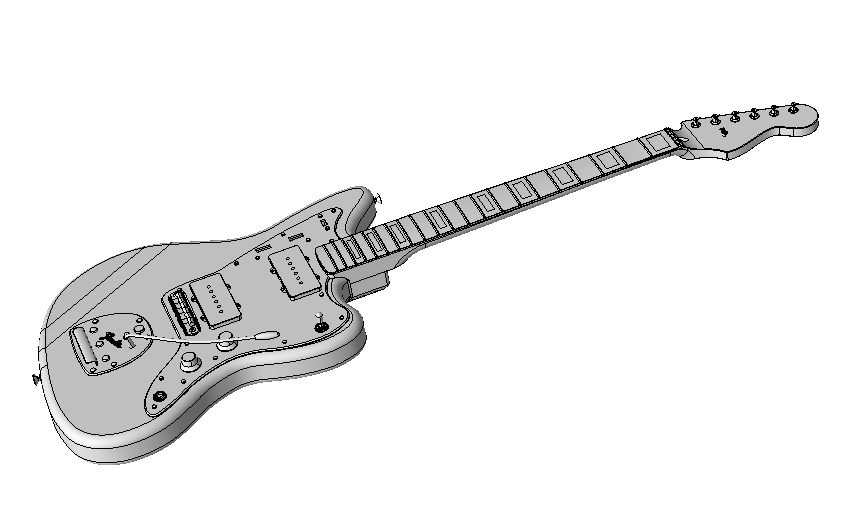
\includegraphics[width=1.0\textwidth]{images/guitarCAD.png}\\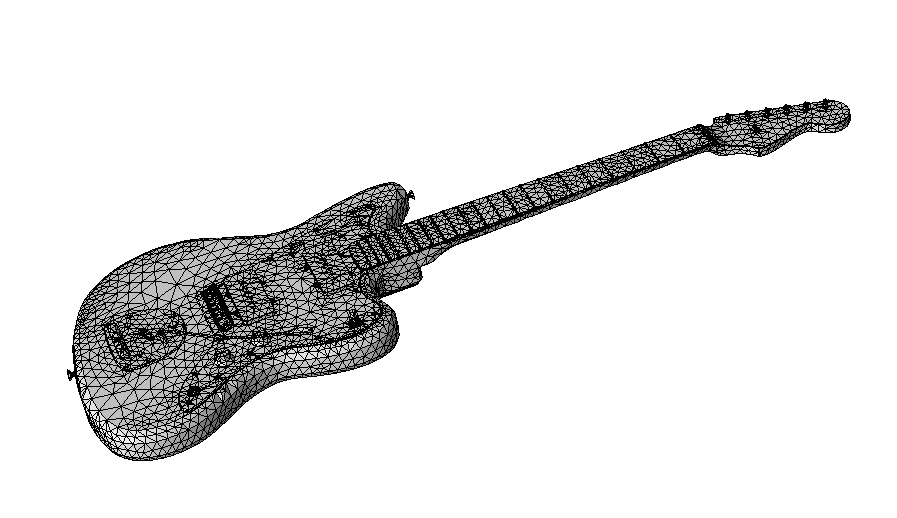
\includegraphics[width=1.0\textwidth]{images/guitarMESH.png}
\caption{Geometry (top) and Mesh (bottom) of a guitar.}
\label{fig:guitar}
\end{figure}
While our application is for the simulation of physical phenomena, meshes are also commonly used for graphics applications, for example, to represent the geometry of objects in video games (resolution is loosely like number of triangles).

For more info, a video (in French) by a former post-doc is up here \url{https://www.rocq.inria.fr/gamma/Frederic.Alauzet/}

\section{Curved Meshes}
Consider the geometry and initial mesh in Figure \ref{fig:initcurv}.
\begin{figure}
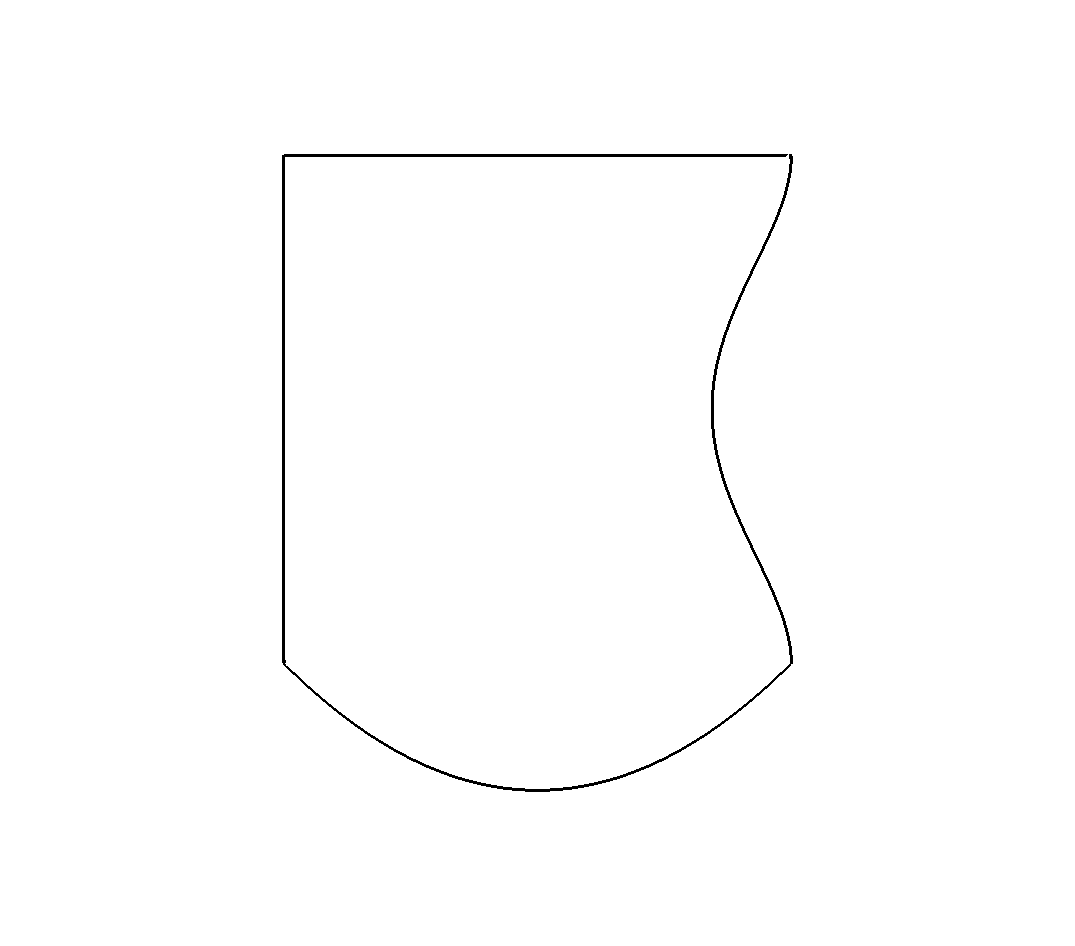
\includegraphics[width=0.5\textwidth]{images/curvedgeom.png}
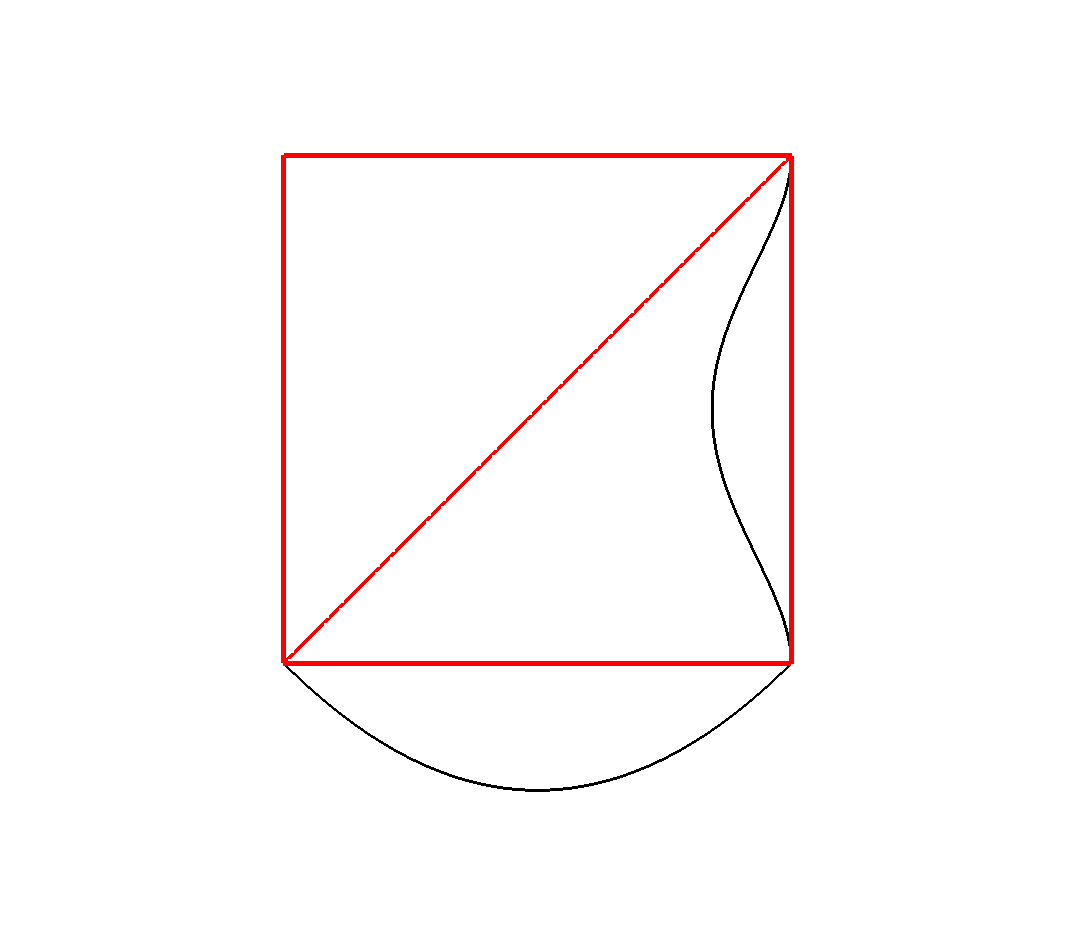
\includegraphics[width=0.5\textwidth]{images/curved1.png}
\caption{Geometry (left) and initial triangulation (right).}
\label{fig:initcurv}
\end{figure}
We can improve our approximation of the geometry in two ways. We can use the conventional approach, and increase the number of trianges. We can also use curved triangles, representing the triangle by a spline or approximate surface, as in Figure \ref{fig:endcurv}.
\begin{figure}
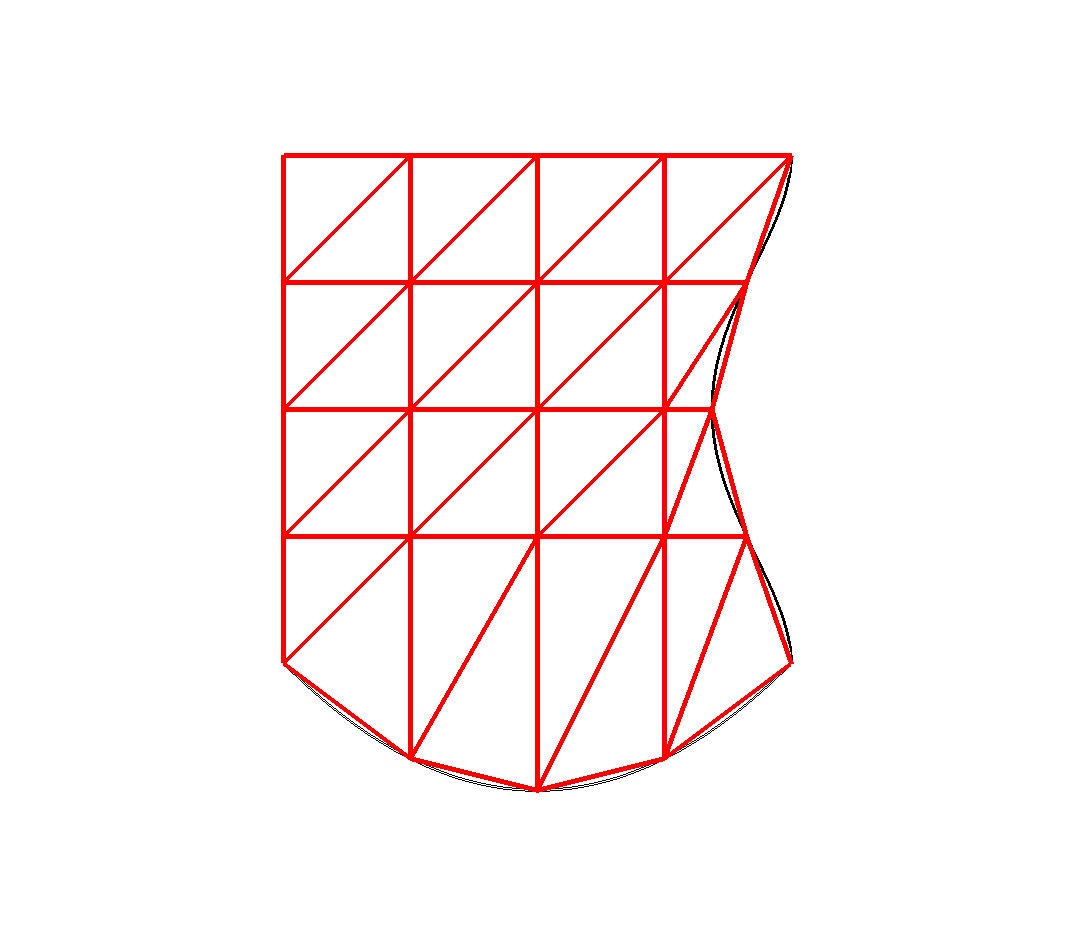
\includegraphics[width=0.5\textwidth]{images/uniform2.png}
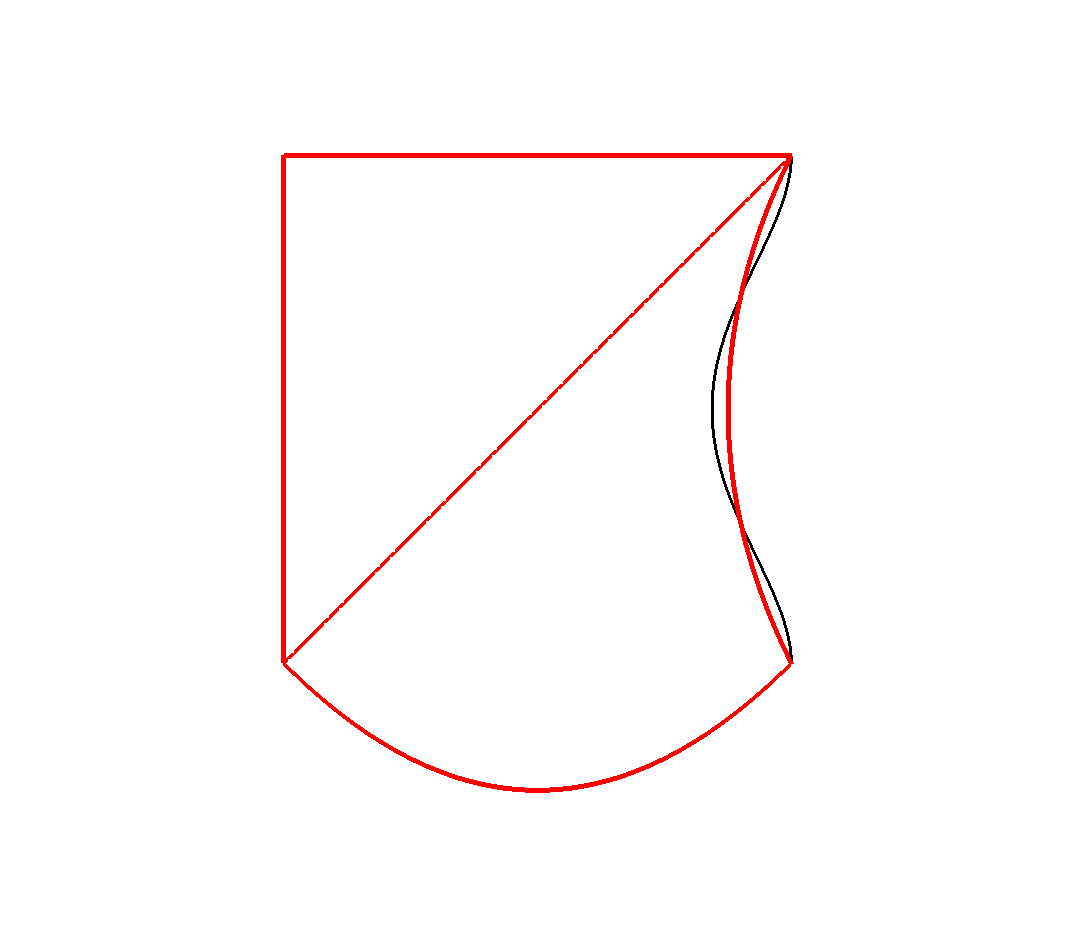
\includegraphics[width=0.5\textwidth]{images/curved3.png}
\label{fig:endcurv}
\caption{Improving by the approximation of the geometry with more triangles (left) and curved triangles (right).}
\end{figure}
This can reduce the number of triangles used to represent the geometry while improving the geometric approximation, reducing simulation time and improving solution accuracy. Unlike their linear counterparts, guaranteeing validity (no self intersections) is a challenge, and determining validity itself is a non-trivial process. As such, we have several ideas for quality checking and verification and understanding curved elements. This project is simple coding and a fair amount of math (splines, curved surfaces, etc) and is a mix of software, algorithms, and geometry. The goal would be to understand these methods and find the best method(s) for analyzing curved meshes. This could also lead to looking at using these estimates to improve mesh quality, and other aspects of curved meshing.
\section{Automatic Differentiation} 
As part of moving the vector/matrix math into its own component, and supporting
work that Brian and I are doing (separate things), we would like to develop our
own automatic differentiation system and integrate that with apf::Vector,
apf::Matrix and so on. It could also be used to make it easier to add shape
functions to APF. Brian would like to be the “mentor” for this student, this
project is a good mix of math and C++ experience.

\url{https://github.com/bgranzow/diff}

\section{ParaView VTK} 
This project involves augmenting the capabilities of our visualization file
output code. We would like to switch from decimal number representations to
binary-exact representations. We would also like to use compression algorithms
on the data to reduce disk usage and improve write speeds. Finally, we would
like to use a directory hierarchy to try to improve write speeds in parallel.

\url{http://www.paraview.org/}

\url{http://www.vtk.org/wp-content/uploads/2015/04/file-formats.pdf}

\url{https://github.com/SCOREC/core/blob/master/apf/apfVtk.cc}

\section{Parameter Studies}
We are developing a new mesh adaptation code, which uses local operations to
modify a mesh until the edges are the desired length and the elements
(triangles for example) are the desired shape. These operations rely on some
parameters like what the minimum acceptable quality is and so on. We would like
to study the variation of both output quality and program runtime on those
parameters, and in particular identify reasons why certain parameters make the
program faster and/or more effective.

\url{https://github.com/ibaned/august}

\section{Porting Python to Modelica} 
We are working with architecture (CASE, the center for architecture science and
ecology) to model dynamic building facades (smart windows). We are currently
modeling one of their systems using an in house python code. This will be
converted into  component in Modelica, a popular tool for analysis of
energy/building systems. This project involves interfacing our model with
Modelica, or possibly working on a GUI or other tools to allow Architecture
researchers/developers to use our models.

\section{Performance Profiling}
Define and implement convenient, low-overhead, portable mechanisms to measure
and compute statistics of run time, memory consumption, and communication data.
Performance data will be collected with identifying meta-data such that human-
and machine- readable output can be produced.  Development will require
writing, debugging, and testing C/C++ data structures with functional
interfaces (API).

\section{GPU Graph Operations}
The Department of Energy is increasingly building machines that have most of
their computing power available in GPUs (link to Titan or something). This
project involves working on a GPU-capable version of a mesh adapt
code. The special thing about this software is it is doing graph operations on
the GPU, which traditionally is not a good fit but we think we have good
algorithms for it. The project specifically involves developing the CUDA
portion of a general-purpose shared memory parallelism system and doing
performance tests on various GPUs, plus performance optimization as necessary.

\url{https://github.com/ibaned/flounder}

\url{https://www.youtube.com/watch?v=vYA0f6R5KAI}

\end{document}
This is never printed
